\documentclass[letterpaper, 10 pt, conference]{ieeeconf}
\IEEEoverridecommandlockouts
% The preceding line is only needed to identify funding in the first footnote. If that is unneeded, please comment it out.
%\usepackage{cite}
\overrideIEEEmargins
\usepackage{iftex}
\ifXeTeX % Times (ptm) is pdfLaTeX-only; use its OpenType clone under XeLaTeX/Tectonic
  \usepackage{fontspec}
  \setmainfont{texgyretermes}[Extension=.otf, UprightFont=*-regular, BoldFont=*-bold,
    ItalicFont=*-italic, BoldItalicFont=*-bolditalic]
\fi
\usepackage{amsmath,amssymb,amsfonts}
\usepackage{algorithmic}
\usepackage{graphicx}
\usepackage{textcomp}
\usepackage{xcolor}
\usepackage{tikz}
\newcommand{\xmark}{%
\tikz[scale=0.23] {
    \draw[line width=0.7,line cap=round] (0,0) to [bend left=6] (1,1);
    \draw[line width=0.7,line cap=round] (0.2,0.95) to [bend right=3] (0.8,0.05);
}}
\newcommand{\cmark}{%
\tikz[scale=0.23] {
    \draw[line width=0.7,line cap=round] (0.25,0) to [bend left=10] (1,1);
    \draw[line width=0.8,line cap=round] (0,0.35) to [bend right=1] (0.23,0);
}}

\def\BibTeX{{\rm B\kern-.05em{\sc i\kern-.025em b}\kern-.08em
    T\kern-.1667em\lower.7ex\hbox{E}\kern-.125emX}}



%%%%%%%%%%%% own packages %%%%%%%%%%%%%%%%%%%%%%
\usepackage{hyperref}
\usepackage{blindtext}
\usepackage{siunitx}
\usepackage{booktabs}
\usepackage{subfig}
\usepackage{todonotes}
\let\labelindent\relax % ieeeconf.cls already defines \labelindent, which clashes with enumitem
\usepackage{enumitem}
\usepackage{float}
\usepackage[backend=bibtex,style=ieee,mincitenames=1,maxcitenames=1,url=false]{biblatex}
\addbibresource{references.bib}
\newcommand{\daa}{Drive\&Act\xspace}
% Auch Abbildung und nicht nur die Nummer wird zum Link (abgeleitet
% aus Posting von Heiko Oberdiek (d09n5p$9md$1@news.BelWue.DE);
% Verwendung: In \abbvref{label} ist ein Beispiel dargestellt
\providecommand*{\figrefname}{Figure~}
\newcommand*{\figref}[1]{%
	\hyperref[fig:#1]{\figrefname{}}\ref{fig:#1}%
}
% ebenso bei Tabellen
\providecommand*{\tabrefname}{Table~}
\newcommand*{\tabref}[1]{%
	\hyperref[tab:#1]{\tabrefname{}}\ref{tab:#1}%
}
% und Abschnitten
\providecommand*{\secrefname}{Section~}
\newcommand*{\secref}[1]{%
	\hyperref[sec:#1]{\secrefname{}}\ref{sec:#1}%
}
% und Kapiteln
\providecommand*{\chaprefname}{Chapter~}
\newcommand*{\chapref}[1]{%
	\hyperref[chap:#1]{\chaprefname{}}\ref{chap:#1}%
}
% und Appendix
\providecommand*{\appendixrefname}{Appendix~}
\newcommand*{\apref}[1]{%
	\hyperref[ap:#1]{\appendixrefname{}}\ref{ap:#1}%
}
% equation
% this overwrites the definition of amsmath which add the same look as the numbering
% of the equation environment including brackets
\providecommand*{\eqrefname}{Equation~}
\renewcommand*{\eqref}[1]{%
	\hyperref[eq:#1]{\eqrefname{}}\ref{eq:#1}%
}
%%%%%%%%%%%% own packages %%%%%%%%%%%%%%%%%%%%%%
\begin{document}

\title{\LARGE \bf 3D Skeleton-based Driver Activity Recognition using Self-supervised Learning}

\author{David J. Lerch$^{1,3}$ \thanks{$^{1}$ David J. Lerch, Manuel Martin and Frederik Diederichs are with the Fraunhofer IOSB, Karlsruhe, Germany
{\tt\small \{firstname.lastname\}@iosb.fraunhofer.de}}, 
Yasser El Bachiri$^{2}$ \thanks{$^{2}$ Yasser El Bachiri is with the Deggendorf Institute of Technology (DIT), Deggendorf, Germany {\tt\small yasser.el-bachiri@stud.th-deg.de}}, Manuel Martin$^{1}$ Frederik Diederichs$^{1}$, Rainer Stiefelhagen$^{3}$ \thanks{$^{3}$ Rainer Stiefelhagen is with the Karlsruhe Institute of Technology (KIT), Karlsruhe, Germany {\tt\small rainer.stiefelhagen@kit.edu}}}

\maketitle

\begin{abstract}
Amidst the increasing integration of technology in car interiors, the risk of driver distraction has become a critical concern for automotive safety. Addressing this issue requires robust methods for detecting driver distractions, often relying on intricate models trained on vast amounts of labeled data. 
However, obtaining such labeled data can be expensive and time-consuming.
In this context, self-supervised learning emerges as a promising approach, leveraging unlabeled data to learn meaningful representations and reduce dependency on annotated datasets.
In this study, we explore self-supervised learning methods for 3D skeleton-based driver activity recognition. We evaluate the performance of our proposed SkelDINO-SAM method across diverse backbone architectures.
Utilizing the Drive\&Act dataset, characterized by its long-tailed distribution of activity classes, we evaluate the effectiveness of our approach in addressing challenges associated with real-world scenarios.
Our findings highlight the superiority of transformer-based backbones, particularly when combined with our SkelDINO-SAM approach. 
Through extensive experiments and ablation studies, we demonstrate the efficacy of our method in enhancing driver secondary task recognition accuracy. 
Overall, our results show the efficiency of our approach outperforming the state-of-the-art method by 11.29\%. Our code is published on \href{https://github.com/davidjlerch/darssl}{GitHub}.
\end{abstract}
\section{Introduction}
In recent years, there has been a growing concern about the increasing number of fatalities caused by car accidents resulting from driver distraction. According to the World Health Organization~(WHO), driver distraction is a major contributing factor to road traffic accidents worldwide. In the U.S., approximately 30\% were observed to perform secondary tasks while driving~\cite{who2011driver}. In the European Union, it's estimated that driver distraction is a contributing factor in 44\% of collisions~\cite{adminaite2021road}.
%Therefore distracted driving has become a leading cause of accidents, accounting for a significant portion of road fatalities worldwide. This alarming trend has necessitated the development of advanced algorithms capable of recognizing driver actions and behaviors to prevent such accidents and promote road safety. 
To address this critical issue, there has been a surge in the development of activity recognition systems specifically tailored for the car interior. These systems aim to identify and analyze various driver activities, such as hand gestures, head movements, and body postures, in real-time. 
%By accurately recognizing these actions, potential distractions and unsafe behaviors can be identified, allowing for timely intervention and accident prevention. 


\begin{figure}[t]
      \centering
      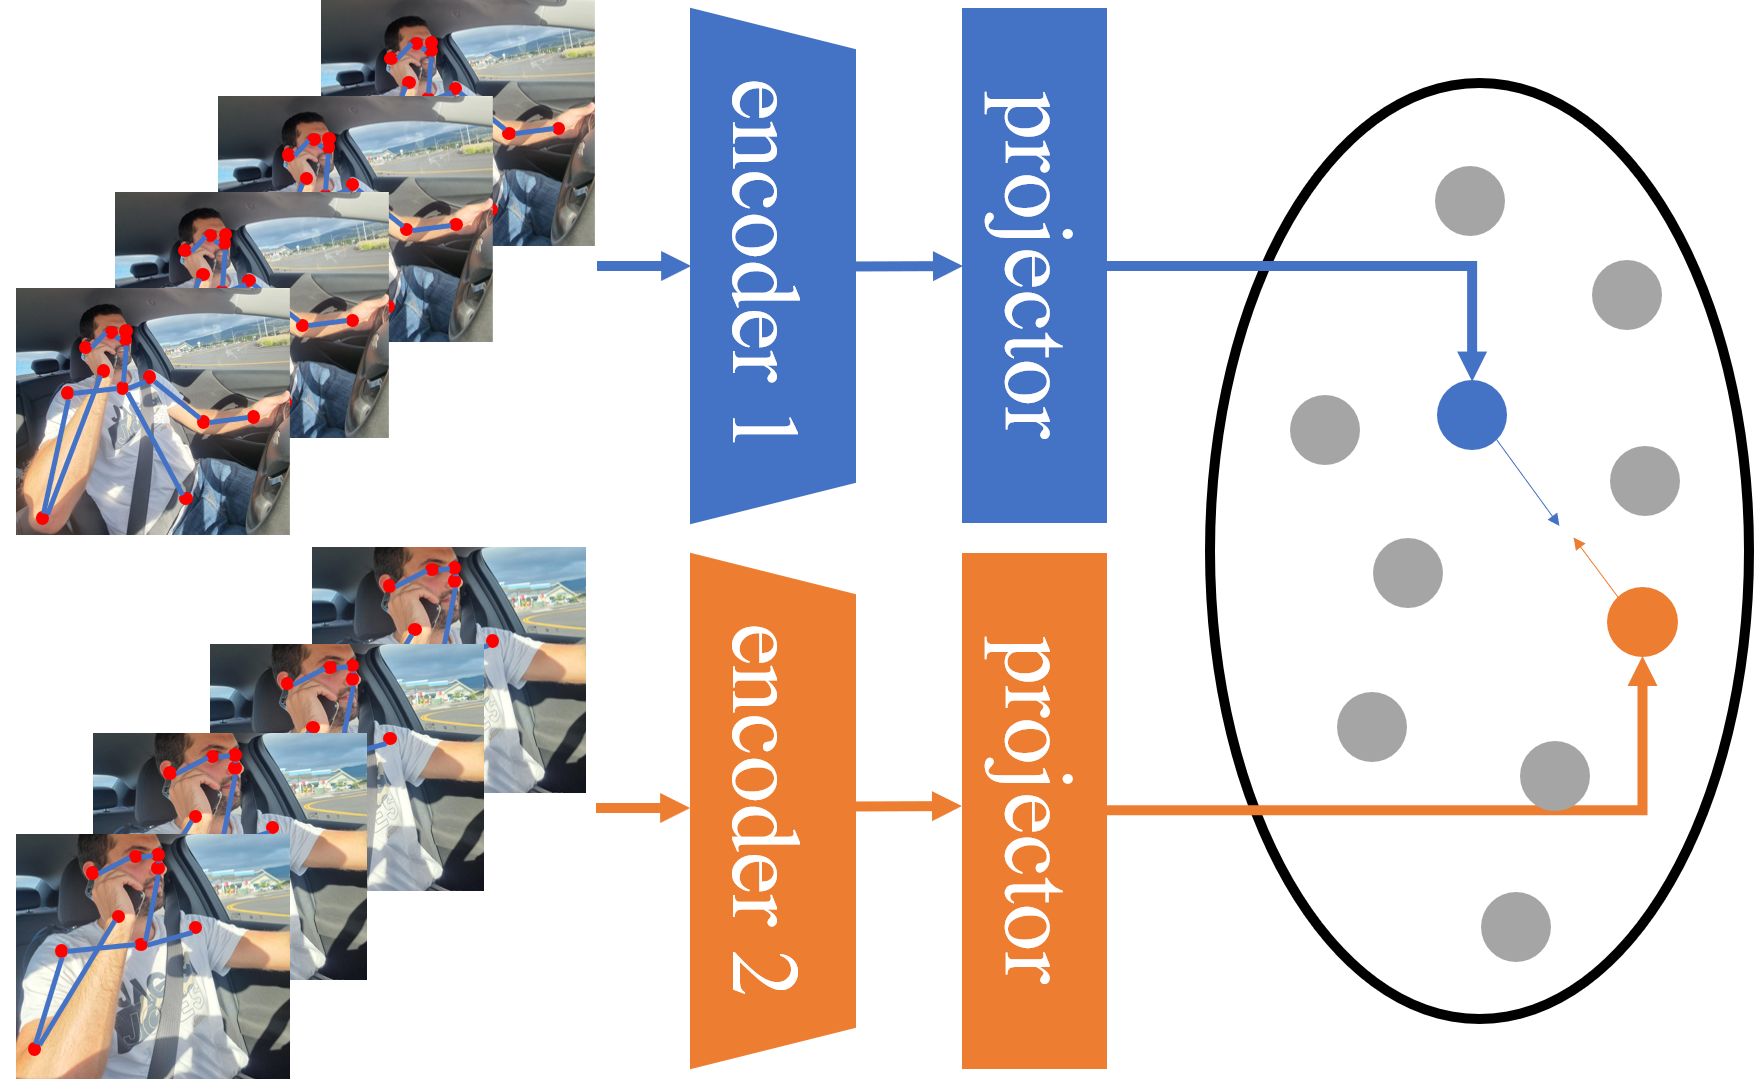
\includegraphics[width=\linewidth]{figures/darssl.png}
      \caption{Principle of a 3D skeleton-based contrastive self-supervised learning approach without negative samples for driver activity recognition. It consists of a two encoders. Different augmentations of the same sample are input to the encoders.}
      \label{fig:darssl}
\end{figure}


Traditional supervised learning methods have been widely employed for activity recognition tasks. However, they heavily rely on annotated datasets, which are costly and time-consuming to produce. 
%Annotated datasets require manual labeling of each action instance, posing practical limitations when it comes to scaling up the training process. To overcome these challenges, self-supervised learning has emerged as a promising alternative approach. 
Unlike traditional supervised learning, self-supervised learning leverages label-free data to learn meaningful representations. In the context of these challenges and opportunities, this study aims to enhance vehicle interior activity recognition by leveraging contrastive self-supervised learning techniques with 3D driver skeleton representations. 
%By utilizing label-free data, this approach can effectively learn informative representations that capture the nuances of driver actions in the car interior. 
Through extensive experimentation and evaluation, we seek to demonstrate the effectiveness of contrastive self-supervised learning with 3D driver skeleton representations in improving the accuracy and robustness of in-cabin activity recognition systems. 

Human activity recognition has been extensively studied using different modalities, such as RGB videos or depth cameras. However, these modalities often come with significant computational costs, making them less suitable for resource-constrained environments. 
%In response to this challenge, human skeleton data has emerged as a promising alternative. 
Skeleton data offers a more efficient representation of human activities, reducing the computational complexity and storage requirements. They also provide a lightweight and efficient alternative that not only reduces computational overhead but also offers the potential to generalize across domains, enabling broader applicability in real-world scenarios. While self-supervised learning has shown promise in various domains, its application to skeleton-based driver activity recognition is still in its early stages. Further research and investigations are necessary to explore the full potential of self-supervised learning in this context. With our work we contribute to this exploration of self-supervised 3D skeleton-based driver activity recognition.

Furthermore, the lack of large activity recognition datasets specifically dedicated to driver behavior inside the car presents another challenge. Existing datasets often focus on general activity recognition but fail to capture the nuanced activities and behaviors specific to drivers within the vehicle environment. To address this gap, we will focus on the test and evaluation on the Drive\&Act dataset \cite{drive_and_act_2019_iccv} tailored specifically to driver behavior inside the car. This dedicated dataset incorporates a wide range of driver activities and behaviors, providing a realistic and comprehensive evaluation platform for activity recognition algorithms in the automotive context. 
%This dataset uniquely facilitates research on activity recognition under realistic driving conditions, incorporating factors like low illumination and limited body visibility. By addressing these practical challenges, our research aims to provide insights into the models' adaptability to real-world scenarios, ultimately contributing to the development of more effective and resilient action recognition systems for in-vehicle environments.
%The first research objective is to design and develop a contrastive self-supervised learning approach specifically tailored for action recognition on 3D human skeleton data. The focus will be on leveraging the benefits of contrastive learning to learn rich and discriminative representations from unannotated skeleton data. 
Our proposed approach is based on the image-based self-supervised self-distillation with no labels (DINO) framework \cite{caron2021emerging}. 
%where a transformer serves as the backbone, which has motivated us to explore its potential for skeleton-based action recognition. Transformers have demonstrated remarkable capabilities in learning meaningful representations from data, especially in self-supervised learning tasks. 
The main contributions of our work are:
\begin{itemize}
\item[1)]
We adopt the image-based DINO approach \cite{caron2021emerging} for skeleton data and propose a SkeletonDINO approach for self-supervised skeleton-based activity recognition.
\item[2)]
We combine this SkeletonDINO approach with the Skeleton Barlow Twins (SkeletonBT) \cite{zhou2023self} to our SkeletonDINO approach with separated augmentation modules (SkelDINO-SAM).
\item[3)]
We perform extensive experiments on self-supervised methods for driver activity recognition. We compare two self-supervised methods Barlow Twins (BT) \cite{zbontar2021barlow} and our SkelDINO-SAM for the three different backbones spatio-temporal graph convolution network (ST-GCN) \cite{yan2018spatial}, spatio-temporal tuple transformer (STTFormer) \cite{qiu2022spatio} and transformer \cite{vaswani2017attention}. We show that our SkelDINO-SAM approach with Transformer backbone outperforms state-of-the-art approach by 11.29\%.

\end{itemize}
%Leveraging the success of transformers in SSL, we propose to use the STTFormer \cite{qiu2022spatio}, a spatio-temporal transformer-based network, as the backbone in our apporach inspired by DINO. Then for our experiments, will implement and evaluate the existing PSTL framework in \cite{zhou2023self}, a partial spatio-temporal learning, and compare it with the DINO approach. The PSTL approach utilizes the spatio-temporal graph convolution network (ST-GCN) by \textcite{yan2018spatial} as the encoder.

%\pagebreak
\section{Related Work}
%\textbf{Activity Recognition with RGB Data:} \textcite{tran2015learning} propose the ”Two-Stream Convolutional Networks” that integrated spatial and temporal streams to capture static appearance and motion information, respectively. This work demonstrated the efficacy of fusing RGB data with optical flow information for activity recognition, achieving state-of-the-art performance on benchmark datasets. The introduction of C3D by \textcite{ji20123d} leverages 3D convolutions to capture spatio-temporal patterns directly from RGB videos, demonstrating superior performance in activity recognition compared to traditional 2D CNNs. Since the introduction of I3D \cite{carreira2017quo}, 3D-CNN has emerged as the standard method for activity recognition. Since then, the activity recognition community has put out several cutting-edge 3DCNN designs \cite{feichtenhofer2020x3d, feichtenhofer2019slowfast} that exceed I3D in accuracy and efficiency.

%Moreover, \textcite{franco2020multimodal} and \textcite{tran2015learning} propose a novel activity encoding method using temporal images from RGB video sequences and integrating complementary information from a skeleton and temporal data. The proposed method outperforms state-of-the-art methods on public datasets. The challenges addressed in this paper include the difficulty of recognizing complex activities with high intra-class variability and the need for robustness to occlusions and noise. These challenges were addressed by using a multimodal approach that combines RGB and skeleton data, as well as a novel activity encoding method that uses temporal images.

\textbf{Skeleton-based activity recognition:} Skeleton data offers a compact and informative representation of human actions, focusing on the spatial arrangement and temporal dynamics of joints.
%Early approaches involved the use of histograms of joint angles or velocities as feature representations~\cite{xia2012view}. By quantizing joint angles or velocities into bins and constructing histograms, these methods attempted to capture the spatial and temporal dynamics of actions. 
With the arrival of deep learning, there was a paradigm shift in skeleton-based activity recognition. Recurrent neural networks (RNN) were amongst the first deep learning methods applied to skeleton based activity recognition \cite{baccouche2011sequential}. RNNs enabled the modeling of temporal dependencies in activity sequences, capturing the dynamics of actions over time \cite{song2017endtoend, wang2017modeling}. Convolutional neural networks (CNN) were adapted to handle skeleton data by treating joint coordinates as image-like representations \cite{du2015skeleton, zhang2019view}. \textcite{zhang2018adding} propose a recursive connection to create a EleAtt-RNN block. They address the challenges of modeling complex sequential information with fixed-weight RNNs and the limitation of existing attention mechanisms that require additional parameters and computational overhead. However, various related methods \cite{wu2014leveraging, zhao2017two} often are unable to achieve a competitive outcome due to the RNN-based architecture’s poor spatial modeling capability.

CNN architectures can effectively handle spatial data, leading to an increased interest in CNNs for skeleton based activity recognition tasks. \textcite{ding2017investigation} investigate encoding richer spatial features into texture color images or 2D pseudo-images for 3D human activity recognition using a CNN-based approach. Each type of feature is encoded into images in two or more ways to further explore the spatio-temporal information. \textcite{liu2017enhanced} investigates methods to enhance skeleton visualization for improved activity recognition under varying viewpoints. On the other hand, GCNs have emerged as a popular choice for effectively representing and processing graph-structured data, including skeleton graphs \cite{shi2019two, cheng2020skeleton, martin_dynamic_2020}. The ST-GCN approach constructs a spatial-temporal graph using joints as graph vertices and incorporating natural connections in both human body structures and time as graph edges.
Since the introduction of ST-GCN, the use of GCNs for skeleton-based activity recognition has garnered significant attention, leading to various related works. \textcite{li2019actional} propose AS-GCN, which does not only recognize a person’s activity but also employing a multi-task learning strategy to predict the subject’s next possible pose.

In skeleton-based driver activity recognition earlier work focused on RNN-based~\cite{drive_and_act_2019_iccv} and GCN-based approaches~\cite{martin_dynamic_2020}. More recent work incorporates attention mechanism with GCN for efficient driver activity recognition~\cite{li2024incomplete}.

The vanilla transformer model~\cite{vaswani2017attention} makes significant strides in natural language processing (NLP) and has since been adopted in various domains. Inspired by the self-attention in computer vision multiple approaches adopted the transformer principle for skeleton-based activity recognition~\cite{qiu2022spatio, wu2022skeletonmae, cheng_hierarchical_2021, kim_global-local_2022}. \textcite{plizzari2021skeleton} introduce a self-attention based approach instead of regular graph convolutions in both spatial and temporal dimensions. 
This replacement of the graph structure of skeleton data by self-attention allows the model to effectively capture dependencies between joints in space and time, leading to improved activity recognition performance.

\textcite{qiu2022spatio} introduce a spatio-temporal tuples transformer (STTFormer). The skeleton sequence is split into multiple patches, and each patch has numerous consecutive frames that are encoded. The link between various joints’ non-consecutive frames is then captured by a self attention module based on spatio-temporal tuples. 
%This model has shown better performance on benchmark datasets when compared to state-of-the-art methods. 

\textbf{Self-supervised skeleton-based activity recognition:} To our knowledge there is no related 3D skeleton-based driver activity recognition method using self-supervised learning. Therefore we focus this related work on self-supervised skeleton-based human activity recognition. Various self-supervised techniques have been developed to leverage the temporal dynamics and spatial information present in skeleton data. \textcite{zheng2018unsupervised} propose a method based on a recurrent encoder-decoder generative adversarial network (GAN) to reconstruct the input skeleton sequence, capturing long-term temporal dynamics and subtle motion patterns. \textcite{su2020predict} introduce an autoencoder for encoding and reconstructing the skeleton sequence, leveraging clustering and nearest neighbor classification for downstream tasks. Existing 3D skeleton-based autoencoders utilize RNN~\cite{su2020predict, wu2022bi, rao_augmented_2021} or transformer backbones~\cite{Lerch_2024_WACV, wu2022skeletonmae}.

\textcite{lin2020ms2l} proposes a multi-task framework (MS2L) for enhancing the understanding of motion and spatial relationships among joints. AS-CAL~\cite{rao_augmented_2021} introduces a momentum long short-term memory (LSTM) based approach to regularize the feature space, while SkeletonCLR~\cite{li20213d} applies a memory bank and cross-view knowledge mining for more comprehensive representations. \textcite{guo2022contrastive} propose AimCLR, relying on powerful data augmentation, and \textcite{zhou2023self} focus on leveraging local relationships between skeleton joints and video frames in their partial spatio-temporal learning (PSTL) approach. This efficient masking strategy is crucial for real-world applications. To the best of our knowledge we are the first to explore self-supervised learning for skeleton-based driver activity recognition. Inspired by the DINO framework~\cite{caron2021emerging}, we propose an adaptation explicitly designed for 3D skeleton data. Our baseline to our proposed method is the PSTL approach \cite{zhou2023self}. PSTL is tested in skeleton-based general human activity recognition.

%\textbf{Self-supervised skeleton-based activity recognition:} Besides the supervised approaches various self-supervised techniques are developed to leverage the temporal dynamics and spatial information present in skeleton data. \textcite{zheng2018unsupervised} propose a method based on a recurrent encoder-decoder GAN to reconstruct the input skeleton sequence. With learning to reconstruct the input sequence, the model can capture long-term temporal dynamics and subtle motion patterns essential for activity recognition. \textcite{su2020predict} introduce a autoencoder to encode and reconstruct the skeleton sequence. For the classification downstream task they use clustering and nearest neighbor classifier. The method leverages both prediction and clustering to encourage the model to learn more discriminative and compact representations. 
%Existing 3D skeleton-based autoencoders are based on RNN \cite{su2020predict, wu2022bi, rao_augmented_2021} or transformer \textcite{Lerch_2024_WACV, wu2022skeletonmae} backbones.
%\textcite{lin2020ms2l} propose MS2L a multi-task framework, including motion prediction and jigsaw puzzle tasks, to enhance the model’s understanding of motion and spatial relationships among joints. \textcite{rao_augmented_2021} introduce AS-CAL, an momentum LSTM based approach to regularize the feature space. \textcite{li20213d} propose SkeletonCLR, which applies a memory bank to store negative samples and employs a cross-view knowledge mining strategy. By leveraging the memory bank and cross-view consistency, the model can capture more comprehensive and discriminative representations. In order to add movement patterns and compel the encoder to acquire broader representations, \textcite{guo2022contrastive} propose AimCLR to make extensive use of augmentation. These contrastive learning approaches significantly rely on powerful data augmentation procedures. 
%While current approaches focus on strong augmentation techniques to discriminate different skeletons, \textcite{zhou2023self} aim to leverage the local relationship between various skeleton joints and video frames in their Partial Spatio-Temporal Learning (PSTL) approach. In the PSTL approach they adopt a unique spatio-temporal masking strategy to construct partial skeleton sequences, allowing the model to focus on the specific regions of interest. The framework utilizes a negative-sample-free triplet stream structure adopted from Barlow Twins (BT) \cite{zbontar2021barlow} for a so-called SkeletonBT, comprising an anchor stream without any masking, a spatial masking stream with Central Spatial Masking (CSM), and a temporal masking stream with Motion Attention Temporal Masking (MATM). This efficient masking strategy is crucial for real-world applications.

%Although this approach works well for general 3D skeleton-based human activity recognition datasets, the performance drops when applied on the car interior domain. Therefore, we propose an approach inspired by the DINO framework \cite{caron2021emerging}. Unlike the original DINO, which focuses on image data, our adaptation is designed explicitly for 3D skeleton data.

%\pagebreak
\section{Method}
In this section, we explore different self-supervised approaches to leverage the benefits of self-supervised learning: we adopt the image-based DINO \cite{caron2021emerging} approach for 3D skeleton data and combine this SkeletonDINO with SkeletonBT \cite{zhou2023self} to our proposed SkelDINO-SAM. 

\subsection{SkeletonDINO}
In our adaptation inspired by DINO \cite{caron2021emerging}, we leverage its self-distillation framework to enhance label-free skeleton-based action recognition. 
Similar to the original DINO concept, our approach employs two encoder models: the student and the teacher network. The primary objective remains for the student to learn robust representations guided by the teacher. Central to this technique is self-distillation, where the teacher network guides the learning process of the student network through cross-entropy loss.

By processing two different random transformations of an input, akin to the approach in DINO with image data, we pass two skeleton sequences through both the student network ($g_{\theta_s}$) with parameters $\theta_s$ and the teacher ($g_{\theta_t}$) network with parameters $\theta_t$. Each network produces a $K$-dimensional feature representation, denoted as $P_s$ and $P_t$, respectively.

To ensure stable and effective learning, these feature representations undergo normalization using softmax operations with temperature parameters, $\tau_s$ for the student and $\tau_t$ for the teacher. This normalization step maintains the features within a desired range for learning and generalization:

\begin{center}
$P_s(x)^{(i)}=\frac{\exp \left(g_{\theta_s}(x)^{(i)} / \tau_s\right)}{\sum_{k=1}^K \exp \left(g_{\theta_s}(x)^{(k)} / \tau_s\right)}$,
\end{center}

The core of the DINO framework lies in the self-distillation process. The teacher is not updated during  back propagation only the weights of the student network are updated based on the cross-entropy loss:

\begin{center}
$\min _{\theta_s} H\left(P_t(x), P_s(x)\right)$
\end{center}

where:

\begin{center}
$H(a, b)=-a \log b$
\end{center}

The aim is to maximise similarity between the student and teacher features by minimizing the cross-entropy loss. A original skeleton sequence $x$ and a noisy augmentation $x_n$ of the original skeleton sequence are passed to both networks. Only the student network receives masked augmentations. Specifically, given a skeleton sequence and a set $V$ of different skeleton augmentations, the loss function is defined to minimize the cross-entropy between the teacher and student features:

$$
\min _{\theta_s} \sum_{x \in\left\{x_1^g, x_2^g\right\}} \sum_{\substack{x^{\prime} \in V \\ x^{\prime} \neq x}} H\left(P_t(x), P_s\left(x^{\prime}\right)\right)
$$

This loss function drives the student to learn meaningful and discriminativ representations by mimicking the knowledge present in the teacher's feature space. A crucial aspect of DINO is the use of exponential moving average (EMA) to update the teacher parameters $\theta_t$. The teacher network learns from the EMA of the student network parameters, resulting in smoother and more consistent updates. This technique stabilizes the learning process and helps the student converge to meaningful representations. 

%The neural network $g$ is composed of a backbone $f$ which is the STTFormer, and a projection head $h$: $g=h\circ f$. The features used in downstream tasks are the backbone $f$ outputs. The projection head comprises of two layers of a multi-layer perceptron (MLP) with a hidden dimension of 512, l2 normalization, and a fully connected layer (Weight Norm) with weight normalization and K dimensions.

Centering \cite{caron2021emerging} is used to prevent one dimension from dominating while encouraging collapse to a uniform distribution, whereas sharpening \cite{caron2021emerging} does the reverse. The use of both processes balances the impact they have. Output sharpening is carried out by setting the temperature $\tau_t$ to a low value in the teacher's softmax normalization. 
This mechanism has been proven to have a similar impact as the negative samples \cite{caron2021emerging} in which it makes the system learn meaningful representations and prevent collapsing to a uniform distribution. 

\subsection{Separated Augmentation Modules}

For the implementation of the separated augmentation modules (SAM) we first adopt weighted masking according to \textcite{zhou2023self}. The process of assigning masked probabilities is as follows: Let \(V_i\) denote the \(i\)-th joint in the skeleton, where \(i \in (1, 2, ..., n)\), and \(n\) is the total number of joints in the skeleton. .

To calculate the masked probability for each joint \(V_i\), the degree \(d_i\) of each joint is first computed, and then the probability \(p_i\) is set as follows:

\[ p_i = \frac{d_i}{\sum_{j=1}^n d_j} \]

where \(d_i\) represents the degree of the \(i\)-th joint, and the denominator \(\sum_{j=1}^n d_j\) ensures that the probabilities are normalized to 1. By using this Central Spatial Masking (CSM)~\cite{zhou2023self}, we focus on masking joints based on their degree centrality, enhancing the encoder's ability to capture a broader range of joint relationships.

In the temporal masking stream, the Motion Attention Temporal Masking (MATM)~\cite{zhou2023self} strategy is introduced to prioritize frames that change quickly. These frames often contain more semantic information about the actions, making them more valuable for learning meaningful representations. To compute the motion \(m \in \mathbb{R}^{C \times T \times V}\) of the sequences, the temporal displacement between frames is calculated as \(m_{:,t,:} = x_{:,t+1,:} - x_{:,t,:}\), where \(x_{:,t,:}\) and \(t\) is the index of the frame.

Next, MATM calculates the overall motion rate of a frame, which serves as the attention weight. The motion rate \(a_t\) for frame \(t\) is computed as follows:

\[ a_t = \frac{(m_t)^2}{\sum_{i=1}^T (m_i)^2} \]

where \(a_t\) represents the motion rate of frame \(t\), and the denominator \(\sum_{i=1}^T (m_i)^2\) ensures that the attention weights are normalized to 1.

Once the attention weights are computed, the top-K attention weights \(a_{t1}, ..., a_{t_K}\) are selected, and the corresponding frames \(x_{t_1}, ..., x_{t_K}\) serve as the key-frames that contain more semantic information about the actions. These key-frames are then masked, and the encoder is encouraged to capture the relationship between the feature from the masked sequence and the anchor feature, which contains the total semantic information.

\begin{figure}[t]
      \centering
      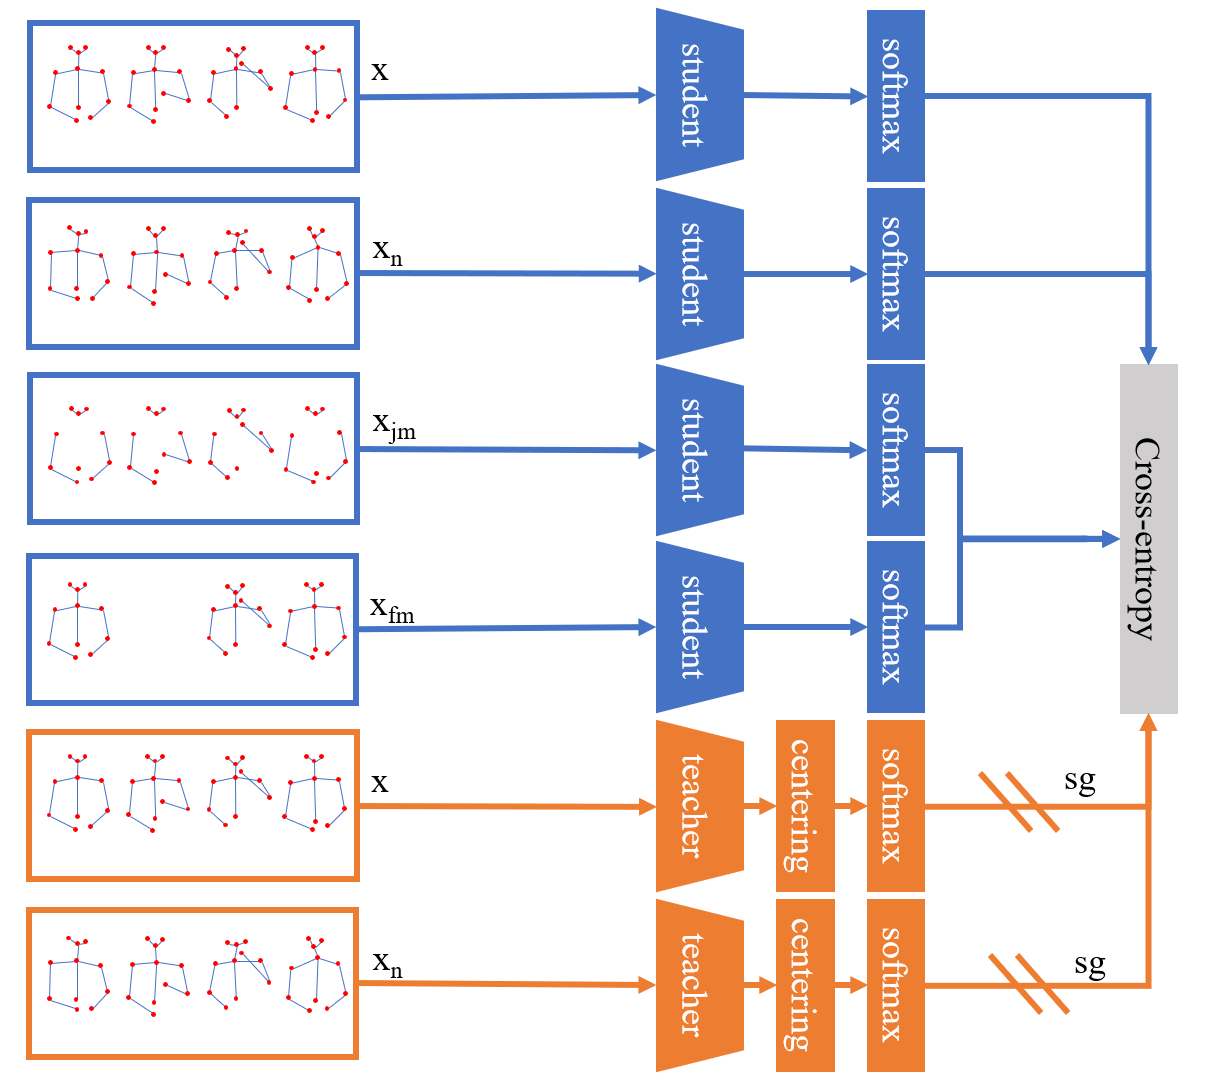
\includegraphics[width=\linewidth]{figures/principle.png}
      \caption{Principle of our SkelDINO-SAM approach. It consists of a student (blue) and a teacher network (orange). The student network receives the original skeleton sequence $x$ and the augmentation with additive noise $x_n$ as well as the frame masked $x_{fm}$ and joint masked sequence $x_{jm}$. The teacher network receives the original skeleton sequence $x$ and the augmentation with additive noise $x_n$.}
      \label{fig:principle}
\end{figure}

\subsection{SkeletonDINO with SAM}
In our SkeletonDINO with SAM (SkelDINO-SAM, see Figure~\ref{fig:principle}), we introduce a novel approach that combines the principles of SkeletonDINO with the concept of SAM, inspired by the work of \textcite{zhou2023self}. Unlike images, skeleton representations are inherently more concise, making them particularly amenable to targeted augmentation strategies. As such, we opt to employ distinct augmentation pipelines for different aspects of the skeleton sequence, rather than applying random augmentations uniformly across the entire sequence.

This approach results in the creation of four distinct inputs for the student network. In addition to the original skeleton sequence, the student network receives variations of the input data, including sequences with additive noise and sequences with joint and frame masking. By diversifying the input data in this manner, we aim to enrich the learning process and enable the student network to better generalize across different types of noise and occlusions.
%For the teacher network input, we adopt a similar strategy, providing both the original sequence and a version with additive noise. This ensures that the teacher network is equipped with diverse training data, allowing it to effectively guide the learning process of the student network while also promoting robustness to various sources of noise and perturbations in the input data.
In the proposed method, the teacher model receives two distinct sets of input data the original skeleton sequence $x$ and the noisy sequence $x_n$. These inputs are embedded by the teacher model. The teacher output embeddings are then centered \cite{caron2021emerging}.

Concurrently, the student model processes multiple sets of input data, including the original skeleton sequence $x$ and the sequence with additive noise $x_n$ as well as the frame masked sequence $x_{fm}$ and the joint masked sequence $x_{jm}$. Each set of data undergoes independent processing within the student model, followed by the application of a softmax function akin to the teacher model. The objective involves comparing the outputs of both teacher and student models using a cross-entropy loss function. Through minimizing this loss, the student model endeavors to approximate the behavior of the teacher model.

%\pagebreak
\section{Experiments}
We now evaluate our SkelDINO-SAM method against other baselines on skeleton-based driver activity recognition tasks. Since our method is designed for label-free pre-training, we evaluate our approach with frozen, self-supervised pre-trained, models. Only for classification, training samples are embedded for nearest neighbor search during testing. We perform ablation studies on different masking probabilities during pre-training as well as linear evaluation and fine-tuning.
\subsection{Dataset}
For our experiments, we evaluate our SkelDINO-SAM method on 
%two different datasets we primarily use the NTU RGB+D \cite{Liu_2020}, a large-scale benchmark for 3D human action recognition for the purpose of achieving the first research objective which is developing and evaluating a contrastive self-supervised approach for action recognition on 3D human skeleton data. 
the Drive\&Act \cite{drive_and_act_2019_iccv} dataset dedicated for driver behavior inside the car. We compare our method to state-of-the-art self-supervised approaches for 3D skeleton-based activity recognition.

%\textbf{NTU RGB+D 60 Dataset:}
%proposed in 2016, was captured simultaneously using three Microsoft Kinect V2 sensors. It comprises 56,000 action sequences in 60 action classes, including 40 daily actions, 9 health-related actions, and 11 mutual actions. The data was collected from 40 volunteers, and each action sequence contains the three-dimensional positions of 25 body joints per frame, as shown in ~\ref{fig:ntu_25joints}. The dataset is divided into training and test sets using two different standards: Cross-Subject (X-Sub) and Cross-View (X-View). In the Cross-Subject setting, the dataset which contains 40320 samples and 16560 samples for training and evaluation, is split based on the person ID, resulting in 20 subsets for both the training and test sets. On the other hand, the Cross-View setting containing 37920 and 18960 samples for training and evaluation, divides the dataset according to camera ID. The samples collected by cameras 2 and 3 are used for training, while those collected by camera 1 are used for testing. Notably, the three cameras have horizontal angles differing by 45° each, ensuring diverse perspectives for robust evaluation.

The Drive\&Act dataset offers a comprehensive collection of driver activities and interactions inside the vehicle cabin, providing valuable insights for driver monitoring and autonomous driving systems. 
%The dataset consists of over 9.6 million frames, recorded from six different camera views and three modalities, collected by five Near-Infrared (NIR) and three RGB-D cameras. The data was recorded using a specially equipped vehicle that was driven on public roads in Germany. The vehicle was outfitted with six synchronized cameras placed in various positions. Three NIR cameras were utilized to capture images in low-light conditions, while three RGB-D cameras were used to capture color images and depth information. The synchronization ensured that all data streams were aligned in time, providing coherent multi-modal information for each frame. 
It includes skeleton data as one of its modalities. Specifically, the dataset includes 3D body and head pose data, which is represented as a time series of 3D rotation matrices. 
%The skeleton data is captured using the OpenPose neural architecture, which is applied to each frame of the dataset that contains the driver's body or head.

The dataset comprises a hierarchical annotation scheme, offering rich semantic information about the driver's behavior. In our experiments we focus on the so called fine-grained activities. These include 34 activities inside the vehicle cabin, such as "adjusting the radio" or "checking the rear-view mirror." Fine-grained activities offer detailed insights into the driver's interactions and behaviors.
%\begin{itemize}
    %\item \textbf{Coarse Tasks:} These represent high-level activities the drivers perform, such as "driving straight" or "turning left." These coarse tasks provide a broader context for understanding the driver's overall behavior.

    %\item \textbf{Fine-Grained Activities:} These include more specific actions inside the vehicle cabin, such as "adjusting the radio" or "checking the rear-view mirror." Fine-grained activities offer detailed insights into the driver's interactions and behaviors.

    %\item \textbf{Atomic Action Units:} This level provides detailed triplets of annotations, including the driver's current action, the object they interact with, and the location of the object. This level of granularity allows for a deep analysis of the driver's actions and intentions.
%\end{itemize}

%The Drive\&Act dataset includes an extensive set of 83 fine-grained activity classes, surpassing previous driver activity recognition datasets by 62 additional activities. This broad range of actions enables a more comprehensive understanding of driver behavior. The dataset's size, with over 9.6 million frames, provides ample data for training and evaluation, making it one of the largest and most diverse datasets for driver activity recognition.

\subsection{Data Preparation and Processing}

Data augmentation is a fundamental aspect of contrastive learning, and it plays a crucial role in generating diverse variations of the input skeleton sequences to enhance the model's ability to learn meaningful representations. In our pre-processing pipeline, we apply various spatial and temporal augmentations, including:

\begin{itemize}
	\item \textbf{Rotation:} An efficient spatial augmentation that randomly rotates the skeleton in all three axes. The rotation angle is in the range [0, 0.35] \si{rad}.
	\item \textbf{Scale:} As a spatial augmentation, scaling is used. The scaling factor is in the range [0.9, 1.1].
    \item \textbf{Spatial masking:} We randomly mask out joints in all frames. Therefore the x, y and z-coordinate of a joint is set to 0 in all frames.
    \item \textbf{Temporal masking:} We randomly mask out frames. Therefore all joint values in a frame are set to 0.
    \item \textbf{Gaussian noise:} We randomly add Gaussian noise with mean 0 and standard deviation 0.01 to the skeleton sequences. 
\end{itemize}

These augmentations are applied to create different variations of the skeleton sequences, enabling the model to capture diverse perspectives of the activities. This leads to more robust and more generalized representations. The rotation and scaling augmentations are used for all input streams including the original sequence. Each input stream is rotated and scaled separate.
In addition to the ordinary augmentations described earlier we utilize weighted masking strategies such as CSM and MATM \cite{zhou2023self}.

We explore the impact of balancing for the Drive\&Act dataset, considering its long-tailed distribution of activity classes. We evaluate the performance of self-supervised learning methods with comparing the recognition accuracies with and without balancing. 
Inspired by \textcite{li2024incomplete} we implement interpolation for incomplete skeleton sequences. The interpolation is a linear interpolation where the available joint positions act as the grid points. For missing joints at the beginning and end of the skeleton sequence we repeat the first and last joint respectively.

\subsection{Implementation Details}

%\textbf{Data processing.} 
%The activity classes in the Drive\&Act dataset follow a long-tailed distribution. Therefore we make use of a balanced sampling strategy to investigate the influence of balancing for the performance of self-supervised learning. For challenging 3D skeleton activity recognition datasets such as Drive\&Act it is crucial to clean the data. Inspired by \textcite{li2024incomplete} we implement interpolation for incomplete skeleton sequences. The interpolation is a linear interpolation where the available joint positions act as the grid points. For missing joints at the beginning and end of the skeleton sequence we repeat the first and last joint respectively.

\textbf{Training details.} The pre-processing in general is label-free. An exception marks the balancing process, where the labels are used in the weighted sampling process. All hyperparameters are determined empirically. We use AdamW optimizer with cosine scheduler for all experiments. The learning rate is linearly ramped up during the first
10 epochs from 0.000001 to 0.001. The weight decay is 0.01 and the batch size 256. For the transformer model we choose the number of encoder blocks to 2 and the hidden dimension to 512.

\textbf{Evaluation protocols.} We calculate the overall accuracy as the mean balanced accuracy of all three splits in the Drive\&Act dataset. For the evaluation of self-supervised learning, we utilized three protocols: linear~(LEP) and 1-Nearest Neighbor~(1-NN) evaluation protocols as well as fine-tuning. For the linear evaluation, we add a linear classifier on top of the frozen pre-trained encoder and then train the classification layer on the target skeleton activity recognition dataset with an initial learning rate of 0.1. In the 1-NN evaluation, we embed all training samples and classify the test samples with a simple 1-NN classifier \cite{su2020predict}. For fine-tuning we train the backbone as well as the linear layer after LEP with an initial learning rate of 0.0001.

\begin{table*}[t]
\begin{center}
\caption{Comparison of SkeletonBT and our SkelDINO-SAM method with different backbones. The test data is classified according to the 1-NN evaluation protocol \cite{su2020predict}. The best score is bold, and the second-best score is underlined.}
\begin{tabular}{c c c c c c c c c}
\toprule
Methods & Backbones & Balancing & Interpolation & Weighted Masking & Split0 & Split1 & Split2 & Accuracy [\%]\\
\hline
Random baseline & & & & & & & & 2.94\\
PSTL* \cite{zhou2023self} & ST-GCN \cite{yan2018spatial} & & & & 15.48 & 15.43 & 13.30 & 14.74\\
\hline
SkeletonBT* \cite{zhou2023self}  & ST-GCN \cite{yan2018spatial} & \xmark & \xmark & \xmark & 14.02 & 15.78 & 12.46 & 14.09\\
  &  & \xmark & \xmark & \cmark & 14.29 & 15.06 & 12.59 & 13.98\\
  &  & \xmark & \cmark  & \xmark & 14.49 & 14.69 & 12.17 & 13.78\\
  &  & \xmark & \cmark  & \cmark  & 14.52 & 15.20 & 12.79 & 14.17\\
  &  & \cmark  & \xmark & \xmark & 16.73 & 17.16 & 13.18 & 15.69\\
  &  & \cmark  & \xmark & \cmark  & 16.65 & 17.07 & 12.48 & 15.40\\
  &  & \cmark  & \cmark  & \xmark & 16.18 & 15.15 & 13.71 & 15.01\\
  &  & \cmark  & \cmark  & \cmark  & 15.72 & 14.97 & 13.20 & 14.63\\
  \hline
SkeletonBT* \cite{zhou2023self} & STTFormer \cite{qiu2022spatio} & \xmark & \xmark & \xmark & 14.73 & 14.24 & 15.10 & 14.73\\
  &  & \xmark & \xmark & \cmark  & 14.70 & 13.89 & 13.80 & 14.13\\
  &  & \xmark & \cmark  & \xmark & 15.41 & 13.06 & 13.05 & 13.84\\
  &  & \xmark & \cmark  & \cmark  & 15.15 & 13.18 & 13.30 & 13.88\\
  &  & \cmark  & \xmark & \xmark & 15.94 & 15.70 & 16.06 & 15.90\\
  &  & \cmark  & \xmark & \cmark  & 16.41 & 14.82 & 16.44 & 15.89\\
  &  & \cmark  & \cmark  & \xmark & 16.00 & 13.51 & 13.79 & 14.43\\
  &  & \cmark  & \cmark  & \cmark  & 16.67 & 14.51 & 14.42 & 15.20\\
  \hline
SkeletonBT* \cite{zhou2023self} & Transformer* \cite{vaswani2017attention} & \xmark & \xmark & \xmark & 22.44 & 23.79 & 20.67 & 22.44\\
  &  & \xmark & \xmark & \cmark  & 23.18 & 24.10 & 20.83 & 22.70\\
  &  & \xmark & \cmark  & \xmark & 22.86 & 22.84 & 20.93 & 22.21\\
  &  & \xmark & \cmark  & \cmark  & 27.92 & 23.44 & 21.24 & 24.20\\
  &  & \cmark  & \xmark & \xmark & 24.61 & 24.39 & 21.06 & 23.35\\
  &  & \cmark  & \xmark & \cmark  & 24.55 & 20.76 & 21.04 & 22.12\\
  &  & \cmark  & \cmark  & \xmark & 29.45 & 23.67 & 21.51 & 24.88\\
  &  & \cmark  & \cmark  & \cmark  & 29.31 & 22.01 & 24.27 & 25.20\\
\hline
SkelDINO-SAM* (Ours)  & ST-GCN \cite{yan2018spatial} & \xmark & \xmark & \xmark & 13.97 & 12.44 & 12.53 & 12.98\\
  &  & \xmark & \xmark & \cmark  & 14.53 & 13.67 & 12.63 & 13.61\\
  &  & \xmark & \cmark  & \xmark & 12.60 & 12.79 & 14.66 & 13.35\\
  &  & \xmark & \cmark  & \cmark  & 13.63 & 14.67 & 12.49 & 13.60\\
  &  & \cmark  & \xmark & \xmark & 15.27 & 13.83 & 12.58 & 13.89\\
  &  & \cmark  & \xmark & \cmark  & 16.24 & 14.15 & 13.53 & 14.64\\
  &  & \cmark  & \cmark  & \xmark & 15.97 & 15.47 & 12.39 & 14.61\\
  &  & \cmark  & \cmark  & \cmark  & 15.33 & 15.26 & 13.66 & 14.75\\
\hline
SkelDINO-SAM* (Ours) & STTFormer \cite{qiu2022spatio} & \xmark & \xmark & \xmark & 14.97 & 14.77 & 15.51 & 15.08\\
  &  & \xmark & \xmark & \cmark  & 15.32 & 16.46 & 15.33 & 15.70\\
  &  & \xmark & \cmark  & \xmark & 16.91 & 14.42 & 13.09 & 14.81\\
  &  & \xmark & \cmark  & \cmark  & 16.14 & 14.92 & 13.94 & 15.00\\
  &  & \cmark  & \xmark & \xmark & 18.29 & 18.36 & 17.69 & 18.11\\
  &  & \cmark  & \xmark & \cmark  & 18.93 & 18.08 & 14.91 & 17.25\\
  &  & \cmark  & \cmark  & \xmark & 18.81 & 16.81 & 16.77 & 17.46\\
  &  & \cmark  & \cmark  & \cmark  & 20.03 & 15.67 & 20.03 & 18.58\\
\hline
SkelDINO-SAM* (Ours) & Transformer* \cite{vaswani2017attention} & \xmark & \xmark & \xmark & 23.47 & 25.06 & 21.21 & 23.25\\
  &  & \xmark & \xmark & \cmark  & 23.52 & 24.99 & 21.19 & 23.23\\
  &  & \xmark & \cmark  & \xmark & 28.71 & 23.61 & 21.59 & 24.64\\
  &  & \xmark & \cmark  & \cmark  & 28.70 & 23.61 & 21.67 & 24.66\\
  &  & \cmark  & \xmark & \xmark & 24.50 & 25.21 & 21.42 & 23.71\\
  &  & \cmark  & \xmark & \cmark  & 24.50 & 25.32 & 21.58 & 23.80\\
  &  & \cmark  & \cmark  & \xmark & 30.53 & 24.31 & 23.10 & \underline{25.98}\\
  &  & \cmark  & \cmark  & \cmark  & 30.58 & 24.27 & 23.23 & \textbf{26.03}\\
\hline
\multicolumn{3}{c}{* these methods and backbones are implemented by ourselves}
\end{tabular}
\label{1NNLEP}
\end{center}
\end{table*}

\begin{table}[t]
\centering
\caption{Experimental results on different joint and frame masking probabilities for SkeletonDINO and SkelDINO-SAM methods with transformer backbone.}
\begin{tabular}{c c c c}
\toprule
Method & Frame Mask & Joint Mask & Acc. [\%] \\
\midrule
SkeletonDINO & 0.80 & 0.5 & 25.87 \\
 & 0.90 & 0.7 & 26.60 \\
 & 0.99 & 0.9 & 26.46 \\
\hline
SkelDINO-SAM & 0.10 & 0.1 & 26.03 \\
 & 0.80 & 0.5 & 26.01 \\
 & 0.90 & 0.7 & \textbf{26.91} \\
 & 0.99 & 0.9 & 26.77 \\
\bottomrule
\end{tabular}
\label{tab:masking_results}
\end{table}

%\pagebreak
\section{Results}

In this section, we present the results of our experiments comparing different methods and backbones (see Table \ref{1NNLEP}) for self-supervised 3D skeleton-based activity recognition without negative samples. 
%Our SkelDINO-SAM method with transformer backbone outperforms the state-of-the-art method PSTL \cite{zhou2023self} by 11.29\%.
%We compare two methods: SkeletonBT and SkelDINO-SAM. We utilize three different backbones: ST-GCN, STTFormer, and Transformer. 
%The results in Table~\ref{1NNLEP} show that our SkelDINO-SAM approach yields the best result for transformer backbone with balancing, interpolation and weighted masking. 
In the following we determine the influence of each component on the final result. Therefore, we calculate the mean difference between the accuracies with and without a certain component.

\subsection{Backbone Performance}

We analyze the performance of different backbone architectures in terms of recognition accuracy. The Transformer backbone outperforms ST-GCN by 9.64\% and STTFormer by 8.27\%. These results highlight the effectiveness of leveraging transformer-based architectures for skeleton-based activity recognition tasks. SkelDINO-SAM combined with STTFormer demonstrates a 1.76\% improvement compared to SkeletonBT, while for Transformer, SkelDINO-SAM yielded a 1.02\% improvement. 

\subsection{Analysis of Components}

We further conduct an analysis of the components within our approach. These components include balancing, interpolation and weighted masking. We show, that all of these components contribute to a higher recognition accuracy. 

\textbf{Balancing} the imbalanced Drive\&Act dataset results in a 1.35\% improvement in recognition accuracy across all methods and backbones. This indicates the importance of addressing class imbalances in the dataset preprocessing stage to improve overall model performance.

\textbf{Linear interpolation} applied to the noisy 3D skeleton data leads to a 0.38\% improvement in recognition accuracy, with a more pronounced effect observed for the Transformer backbone, where the improvement reaches 1.65\%. These results underscore the importance of preprocessing techniques such as interpolation in enhancing the quality of input data for skeleton-based activity recognition models.

\textbf{Weighted masking} of the 3D skeleton data leads to a modest overall improvement (0.17\%), SkelDINO-SAM exhibited a slightly higher improvement of 0.25\%. These results suggest that while masking techniques may provide some benefit, their impact on model performance may vary depending on the specific architecture and dataset characteristics.

\begin{table}[t]
\centering
\caption{Performance comparison of linear evaluation (LEP) and fine-tuning for different backbones. All accuracy values are in~[\%]}
\label{tab:LEP-FT}
\begin{tabular}{c c c c c c}
\hline
Protocol & Backbone & Split 0 & Split 1 & Split 2 & Average \\
\hline
Supervised & ST-GCN & 48.46 & 43.83 & 41.81 & 44.70 \\
 & STTFormer & 50.38 & 42.14 & 40.60 & 44.37 \\
 & Transformer & 52.28 & 44.22 & 40.71 & 45.74 \\
\hline
LEP & ST-GCN & 23.13 & 21.86 & 21.27 & 22.09 \\
 & STTFormer & 32.83 & 27.84 & 23.85 & 28.17 \\
 & Transformer & 34.52 & 26.05 & 25.05 & 28.54 \\
\hline
Fine-tuning & ST-GCN & 45.39 & 44.69 & 40.52 & 43.53 \\
 & STTFormer & 54.60 & 45.93 & 44.76 & 48.43 \\
 & Transformer & 53.68 & 46.97 & 45.16 & 48.60 \\
\hline
\end{tabular}
\end{table}

\subsection{Ablation Studies}

The experimental evaluation conducted on the SkeletonDINO and SkelDINO-SAM methods involves varying probabilities of frame and joint masking. Table~\ref{tab:masking_results} summarizes the results obtained from this evaluation. Our SkelDINO-SAM outperforms the SkeletonDINO baseline for various different masking probabilities. These results demonstrate the effectiveness of SkelDINO-SAM in learning from masked data, with a notable improvement in accuracy compared to SkeletonDINO across different masking probabilities.
Our experiments on LEP in Table \ref{tab:LEP-FT} show a notable improvement for all backbones compared to the 1-NN classification results (see Table \ref{1NNLEP}). When fine-tuned, the models with STTFormer and Transformer backbones outperform even the supervised trained models. 
%These results underline the importance of pre-training indicating the quality of self-supervised learned features.

\subsection{Discussion}
The objective of this study is to examine the efficacy of diverse self-supervised methodologies for 3D skeleton-based activity recognition. This study compares the performance of SkeletonBT and our proposed SkelDINO-SAM method across a range of backbone architectures. 

Our analysis demonstrates that the Transformer backbone consistently outperforms ST-GCN and STTFormer, thereby substantiating the efficacy of transformer-based architectures for such tasks. Moreover, when combined with SkelDINO-SAM, the Transformer backbone demonstrated the highest recognition accuracy, indicating the synergistic benefits of our proposed method and transformer-based backbones.

An examination of the constituent elements of our approach reveals the enhancements attained through the application of balancing, interpolation, and weighted masking techniques. The balancing of the imbalanced dataset resulted in a notable 1.35\% improvement in activity recognition accuracy, which serves to underscore the importance of addressing class imbalances in dataset preprocessing, even in the context of self-supervised learning. Our SkelDINO-SAM method demonstrates superior performance to the state-of-the-art PSTL approach, achieving an accuracy improvement of 11.29\% on the Drive\&Act dataset.

Our ablation studies conducted on SkeletonDINO and different noise levels indicate the benefit of SAM. The results of linear evaluation provide additional insights into the performance and robustness of our approach.

\section{Conclusion}
This paper introduces a self-distillation framework with separated augmentation modules, designed specifically for skeleton data. The results of our experiments demonstrate the effectiveness of our SkelDINO-SAM method for self-supervised 3D skeleton-based driver secondary task recognition, particularly when paired with transformer-based backbones. Our SkelDINO-SAM method demonstrates superior performance compared to the state-of-the-art PSTL approach \cite{zhou2023self}, achieving an improvement of 11.29\%. Our findings highlight the significance of pre-processing techniques and the potential of integrating self-supervised learning with transformer backbones, ultimately leading to enhanced recognition accuracy in challenging 3D skeleton-based driver activity recognition tasks. Subsequent research will assess the efficacy of SkelDINO-SAM in multi-modal models.

% \addtolength{\textheight}{-12cm}

\section*{Acknowledgment}
The work has been funded under the funding codes 19A21031E, 19A21031F
and 19A21031L by the Federal Ministry for Economic Affairs and Climate Action of Germany
(BMWK) on the basis of a decision by the German Bundestag and by the European Union. The
work was performed in the project KARLI (www.karli-projekt.de).

\printbibliography

\end{document}
